% To add an image or include a .tex file you need to add
% \CWD
% to the relative (to the main document) path.
%
% Example:
% \begin{figure}
%   \centering
%   \includegraphics{\CWD/images/example.pdf}
% \end{figure}

Um sapo está no pântano, na frente de um rio. No rio há $N$ vitórias-régia, organizadas em uma sequência. O sapo sabe que, ao pular da vitória-régia $A$ para a vitória-régia $B$, a $A$ afunda para sempre no rio. Além disso, cada vitória-régia é de duas formas: {\tt L}, se dela é possível pular apenas para a esquerda (ou para fora do rio), ou {\tt R}, se dela é possível pular apenas para a direita (ou para fora do rio).

O sapo, então, por diversão, itá escolher uma das vitórias-régia, pular nela, e depois pular para as outras, respeitando a restrição de cada vitória-régia. Em cada pulo, ele pula para a vitória-régia mais próxima na dada direção que ainda não afundou. O sapo quer afundar todas as vitórias-régia dessa maneira, e, depois, pular para fora do rio.

\begin{figure}[H]
  \centering
  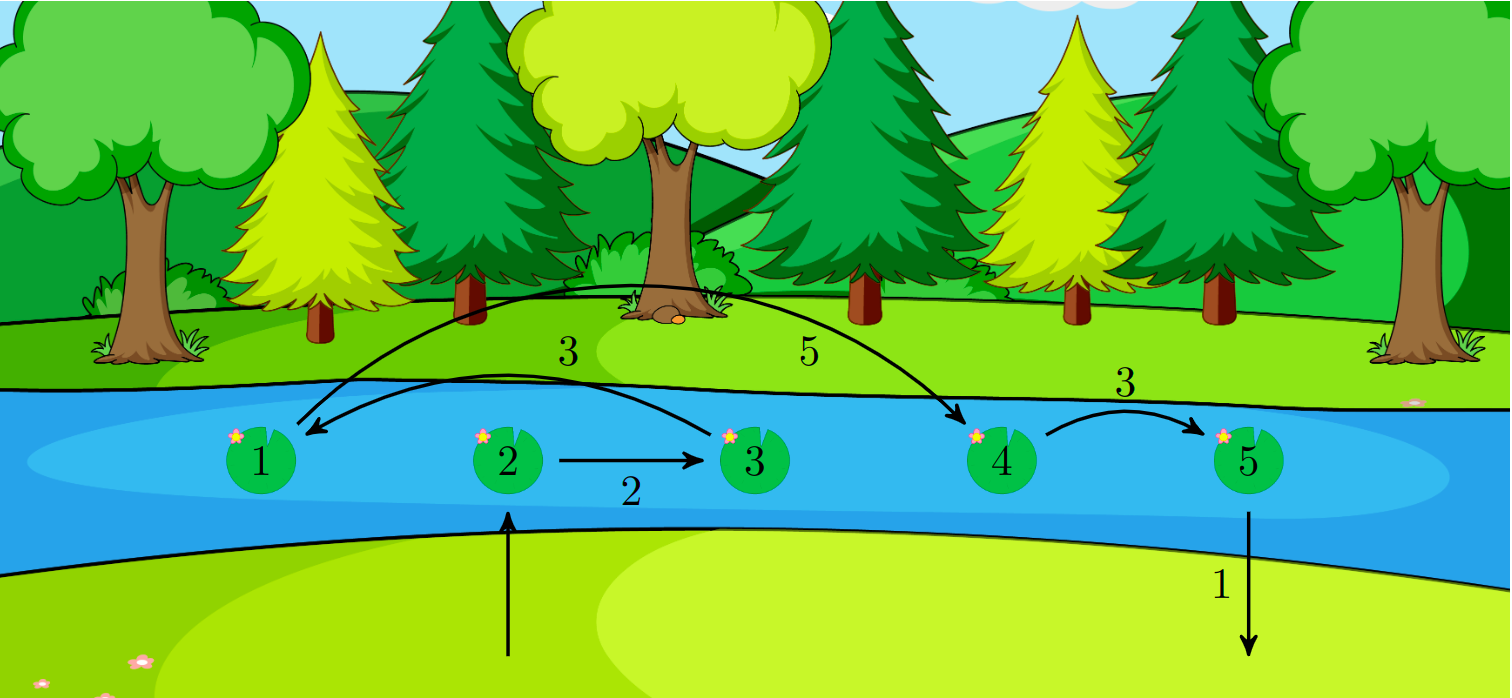
\includegraphics[scale=0.3]{\CWD/image.png}
  \caption{Exemplo para {\tt RRLRL}. Nesse caso, a sequência de vitórias-régia é 2, 3, 1, 4, 5.}
\end{figure}

Ajude o sapo a descobrir alguma sequência de vitórias-régia que satisfaz o que ele deseja, ou fale que isso é impossível.

%
% For input, use one of the following
%
\inputdesc{A primeira linha da entrada contém um inteiro $N$, a quantidade de vitórias-régia no lago. A segunda linha contém um string de $N$ caracteres, cada um deles é {\tt L} ou {\tt R} dependendo se a vitória-régia só admite pulo para a vitória-régia da esquerda ou direita, respectivamente.}

%
% For output, use one of the following
%

\outputdesc{Imprima uma sequência de índices que descreve uma sequência de pulos que o sapo deseja. Se nenhuma tal sequência existir, imprima $-1$.}

%\sampleio will look for files named sample-n.in and sample-n.sol (where n is 1, 2, 3...)
%in the documents directory and include them as samples.

\sampleio
